


\section{Camflow}
We have given a little introduction to Camflow in the previous sections. The Camflow[6] builds upon and learns from previous
OS provenance capture mechanisms, namely PASS, Hi-Fi,
and LPM. The provenance data is captured through Linux
Security Module hooks and NetFilter hooks. The provenance data is transferred to the user space through relayfs,
where it can be stored or analysed. Applications can enrich system level provenance with application-specific details
through a pseudo-file interface. The provenance capture can
be tailored to suit the needs of the application. This is
done through pseudofiles and restricted to the owners of the
capability CAP\_AUDIT\_CONTROL. Camflow provides a library that,
through an API, abstracts interactions with the pseudo-files
and relayfs. This is shown in Fig. 3. 
\vskip 0.1in
CamFlow records how information is exchanged within a system
through system calls. Some calls represent an exchange of information at a point in time e.g., read, write; others may create shared
state, e.g., mmap. The former can easily be expressed within the
PROV-DM model, the latter is more complex to model.
Fig 7 gives an example of whole-system provenance capture example. We can see that Fig. 7 build on the previous work which is illustrated in Fig 4. Fig 4. displays the working of a LSM hook for an 'open' system call. Fig. 7 displays the open system call, however this time, it captures the information and then tailors the information as explained above.
\begin{figure}
	\centering
	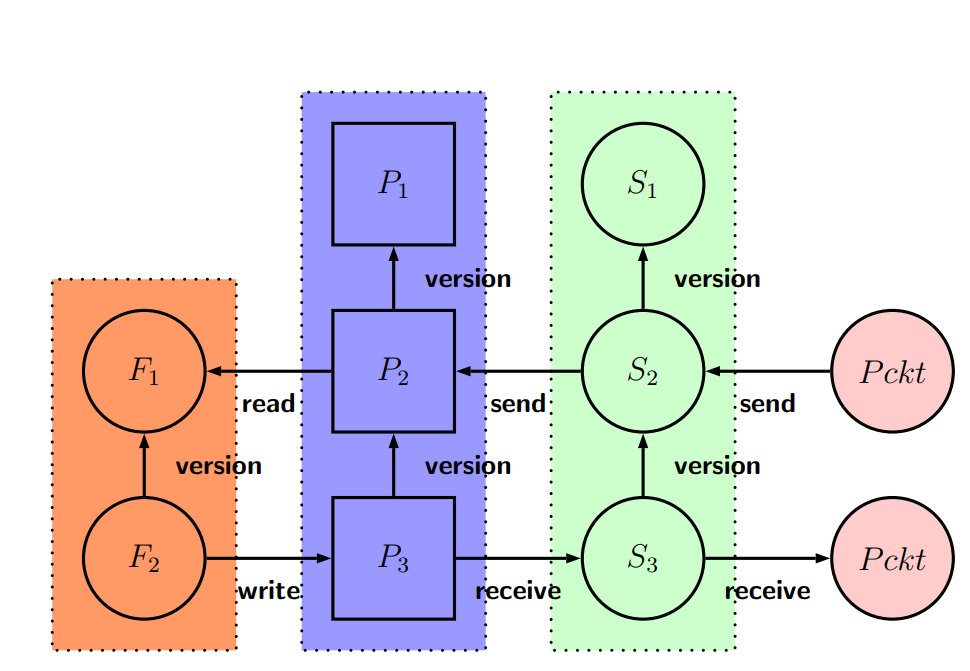
\includegraphics[width=0.7\linewidth]{provenance-g}
	\caption{An example of a provenance graph. CamFlow-Provenance partial graph example. A process P reads information from a file F, sends the information
		over a socket S, and updates F based on information received
		through S}
	\label{fig:provenance-g}
\end{figure}

\begin{figure}
	\centering
	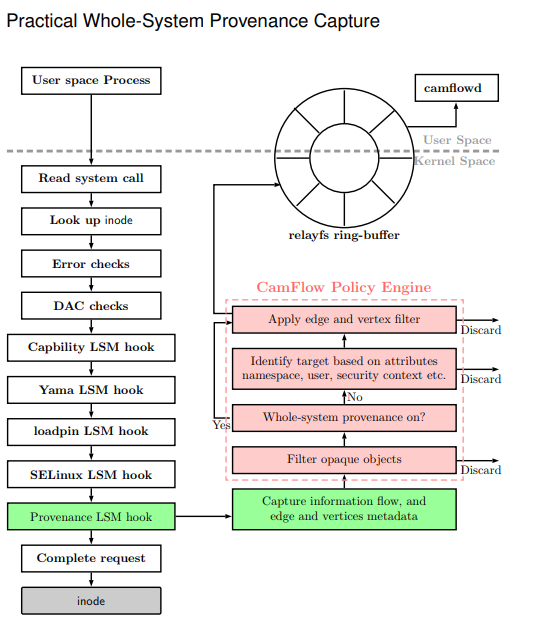
\includegraphics[width=0.7\linewidth]{provenance-capture}
	\caption[open system call]{Executing an open system call. In green is the capture mechanism. The pink is the provenance tailoring mechanism.}
	\label{fig:provenance-capture}
\end{figure}
\subsection{Provenance Data Model}
As explained in the previous sections according to W3C standards the provenance is defined as a directed acyclic graph(DAG). Fig 6 represents an example of a provenance graph. A process P reads information from a file F, sends the information
over a socket S, and updates F based on information received
through S.
\vskip 0.1in 
Provenance graphs are acyclic. A central concept of a CamFlow
graph is the state-version of kernel objects, which guarantees that
the graph remains acyclic. A kernel object (e.g., an inode, a process
etc.) is represented as a succession of nodes, which represent an object changing state. We conservatively assume that any incoming
information flow generates a new object state. Nodes associated
with the same kernel object share the same object id, machine id,
and boot id (network packets follow different rules described in
§ 4.2). Other node attributes may change, depending on the incoming
information (e.g., setattr might modify an inode’s mode). Fig. 6 illustrates CamFlow versioning.
\vskip 0.1in
ig. 3 illustrates CamFlow versioning.
In Fig. 6, we group nodes belonging to the same entity or activity
(F, P and S), based on shared attributes between those nodes (i.e.,
boot\_id, machine\_id, and node\_id). In the cloud context,
those groups can be further nested into larger groups representing
individual machines or particular clusters of machines. For example,
when trying to understand interactions between Docker containers we can create groups based on namespaces (i.e., UTS, IPC,
mount, PID and network namespaces), control groups, and/or security contexts. The combination of these process properties differentiate processes belonging to different Docker containers. Provenance
applications determine their own meaningful groupings.

\subsection{Capture mechanism}
Provenance observed at the system layer may not be sufficient
for all use cases. It may be necessary to disclose to the provenance infrastructure the inner workings of a process. PASS was
the first system to introduce the possibility for an application
to disclose provenance to complement provenance observed at
the OS level, and we implement a similar mechanism. However, this process is complex and generally requires engineering
effort. To accommodate legacy applications we provide an additional
mechanism to annotate the system provenance graph with log
information (as illustrated in Fig. 2). Past research has demonstrated that internal provenance of, for example, web-servers
can be derived from their logs. Therefore, we can understand an application’s inner workings without complex modifications.

\subsection{Provenance graphs show and tell}
The original goal is to eventually make sure that any actions made by a process and that have influence on the system are represented in the graph. The reason we want this to be the case is so that we can detect violations. Based on the previous analysis we have shown that upon adding two new hooks, we get the assurance that all information flows pass through LSM hooks. According to the example in Fig 7, we observe that CamFlow is stacked on all the different modules, which are the Capability LSM hook, Yana LSM hook etc. Every implementation captures different flows and we have explained this in the previous sections. The provenance LSM hook is the lowest in the stack after all the policy stacks. Based on the architecture proposed by Camflow, if the information flows pass through the LSM hooks, the data is indeed getting captured. If all the data is being collected, and no selective capture mechanisms as explained before are being employed we can make get the surety that it shows up on the graph. This is the first part of this part.
\vskip 0.1in
\subsubsection{Property 2}\textit{(Whole system provenance)}
\vskip 0.1in
Iff the Property 1 holds, which means that all information flows pass through the LSM hooks, then CamFlow captures all the data. 

\subsubsection{Theorem 1}\textit{Transitivity}
\vskip 0.1in
If an implementation $\Gamma_1$ adapted for LSM  captures information $\gamma$ and another implementation $\Gamma_2$ is a superset of $\Gamma_1$ then $\Gamma_2$ captures the information $\gamma$